\documentclass[convert={outfile=\jobname.png}]{standalone}
\usepackage{base}

\begin{document}

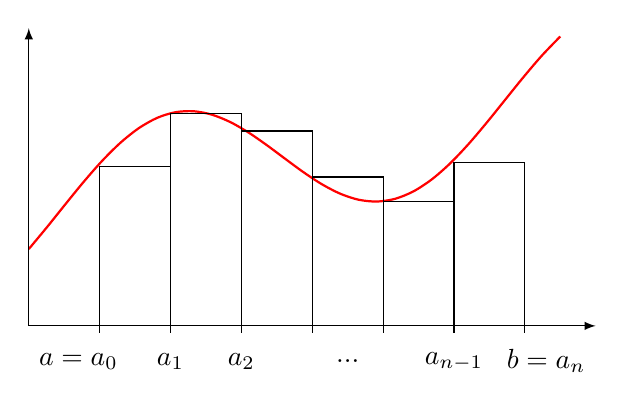
\begin{tikzpicture}[scale=.9]
    \draw[thick, red, smooth,samples=30,domain=2:9.5] plot(\x,{cos(( \x - 4 ) r) + \x/4 - 1});
    \draw[->,>=latex] (2,-2) -- (10,-2);
    \draw[->,>=latex] (2,-2) -- (2,2.2);
    \node at (2.7, -2.5) {$a = a_0$};
    \draw (3, -2.1) to (3, -1.9);
    \node at (9.3, -2.5) {$b = a_n$};
    \draw (9, -2.1) to (9, -1.9);
    \draw (3, -2.1) to (3, .25) to (4, .25) to (4, -2.1);
    \node at (4, -2.5) {$a_1$};
    \draw (4, -2.1) to (4, 1) to (5, 1) to (5, -2.1);
    \node at (5, -2.5) {$a_2$};
    \draw (5, -2.1) to (5, .75) to (6, .75) to (6, -2.1);
    \node at (6.5, -2.5) {$...$};
    \draw (6, -2.1) to (6, .1) to (7, .1) to (7, -2.1);
    \draw (7, -2.1) to (7, -.25) to (8, -.25) to (8, -2.1);
    \node at (8, -2.5) {$a_{n-1}$};
    \draw (8, -2.1) to (8, .3) to (9, .3) to (9, -2.1);
    \end{tikzpicture}

\end{document}
